\documentclass{article}
\usepackage{polski}
\usepackage[utf8]{inputenc}
\usepackage{hyperref}
\usepackage[breakable, most]{tcolorbox}
\tcbset{
    breakable,
    frame code={}
    center title,
    left=0pt,
    right=0pt,
    top=0pt,
    bottom=0pt,
    colback=gray!10,
    colframe=white,
    width=\dimexpr\textwidth\relax,
    enlarge left by=0mm,
    boxsep=5pt,
    arc=0pt,outer arc=0pt,
    }
\usepackage[
backend=biber,
style=alphabetic,
sorting=ynt
]{biblatex}
\addbibresource{bibliography.bib}
\usepackage{graphicx}
\graphicspath{ {./assets/} }
\hypersetup{
    colorlinks,
    citecolor=black,
    filecolor=black,
    linkcolor=black,
    urlcolor=black
}

\title{
    WMI Adventure - grywalizacja studiowania Informatyki \\
    \large Zarządzanie projektem i metodyka zwinna
    }
\author{Marcin Kostrzewski}
\date{22 Listopada, 2021r}

\begin{document}

\maketitle
\newpage
\tableofcontents
\newpage


\section{Wstęp}

\subsection{Streszczenie}
Zarządzanie projektami informatycznymi zaczęło mnie interesować już na 3 roku studiów, gdzie miałem przyjemność uczestniczyć w zajęciach z Inżynierii Oprogramowania prowadzonych przez
dr. Krzysztofa Krzywdzińskiego, w grupie zajęciowej u dr. Patryka Żywicy. WMI Adventure, będący pierwszym większym projektem który realizowałem zespołowo, byłem w dużym stopniu odpowiedzialny za
proces który implementowaliśmy.

Napisałem tę pracę korzystając ze zdobytej wcześniej wiedzy między innymi na zajęciach uczelnianych, z przeczytanych książek,
oraz z doświadczenia zdobytego podczas WMI Adventure. Omawiam w niej różne metodyki zwinne, porównuje je do dawnego, kaskadowego podejścia przedstawiając ich tło historyczne. Przedstawiam też cały proces w WMI Adventure, wykorzystaną metodykę i narzędzia wspomagające.

\subsection{Tematyka}
Organizacja pracy projektowej w zespołach jest kluczowa dla kontrolowanego i przewidywalnego rozwoju, w tym przypadku, oprogramowania komputerowego. W systemach o mniejszym stopniu skomplikowania
i jednoosobowej sile roboczej wystarczy "tylko programowanie". W miarę poszerzania skali projektu i zwiększania ilości członków zespołu, wytwarzanie oprogramowania staje się chaotyczne i niekontrolowane.

Klient, dla którego realizowany jest projekt potrzebuje wspomnianej przewidywalności. Chce chociażby wiedzieć, ile czasu potrwa realizacja jego zlecenia i przede wszystkim jaki będzie jego koszt. Zespół nie jest w stanie
rejestrować postępu prac. Każdy z członków ma inną wizję projektu i priorytetuje zupełnie inne rzeczy, niż te, które są faktycznie istotne dla klienta. Nie wiadomo, nad czym zespoł w danej chwili pracuje.

Potrzeba zatem pewnej struktury, która sprawi, że rozwój oprogramowania będzie przewidywalny - tym właśnie jest zarządzanie projektem, a metodyki to zbiór pewnych ram, które ułatwią jego rozwój.

\subsection{Cel}
Projekt WMI Adventure wykorzystałem do nauki zarządzania zespołem w praktyce. Analizując skutki które przynosiły moje (i innych członków zespołu) decyzje, starałem się z każdym tygodniem usprawniać
proces, wynosząc przy tym doświadczenie i  wiedzę, którą chcę tutaj przekazać.

W litetaturze czy materiałach dostępnych w internecie możemy znaleźć ogólne zasady zarządzania projektem, które też tutaj przytaczam, natomaist
meritum pracy znajduje się w opisie konkretnego wykorzystania tych zasad w oparciu o WMI Adventure, które omawiam w jej drugiej części.

Zespół WMI Adventure liczył początkowo 4 członków, końcowo trzech. Koordynacja mniejszymi zespołami wcale nie musi być prostsza niż tymi dużymi. Chcę w tej pracy opisać metodyki w oparciu o małe zespoły i dostarczyć informację na temat problemów i potencjalnych rozwiązań, które w takich zespołach
występują.

\section{Metodyki pracy i ich kontekst historyczny}
Metodyka pracy to pewien zbiór zasad, które określają w jaki sposób zespoł ma realizować swoje cele. Droga do osiągnięcia tych celów jest skomplikowana i wymaga koordynacji i zarządzania. Metodyka odpowie nam na takie pytania jak: Jaką strukture ma tworzyć zespół? Na jakie role podzielony jest zespół i jakie są odpowiedzialności poszczególnych ról? Jak mierzyć postęp w projekcie? Jak zbierać wymagania projektowe od klienta? Jak wygląda cykl życia projektu? W jaki sposób zarządza się ryzykiem?

Wybór metodyki ma zatem ogromny wpływ na pracę zespołu - sposobów na zrealizowanie jednego celu może być nieskończenie wiele, każdy ma swoje konsekwencje i może doprowadzić do jego pomyślnego ukończenia, lub do całkowitej porażki. Przypadek, w którym nie zastosujemy żadnych schematów i będziemy po prostu programować według własnych zasad też jest w pewnym sensie metodyką, wcale nie skazaną na porażkę.

Metodyka pracy mówi nam zatem \textit{jak} wytwarzać oprogramowanie.

\subsection{Metody kaskadowe}
Początki korporacyjnego świata projektów informatycznych wykorzystywały metody zwane ogólnie kaskadowymi. Mogły wywodzić się z doświadczenia inżynieryjnego zdobytego w fabrykach\cite{scrum}. Linia produkcyjna w fabryce jest
stałym elementem i nie jest odporna na zmiany. Półprodukt przechodzi z jednej linii do drugiej. Nie ma możliwości, żeby gotowy przedmiot opuścił fabrykę bez przejścia każdego etapu bez jakiejkolwiek porażki.
Każdy błąd popełniony przez pracowników na linii produkcyjnej jest katastrofalny i nie jest tolerowany.

Metody kaskadowe w projektach informatycznych działają podobnie - zespół nie jest przystosowany na zmiany, zakładane jest, że wymagania projektowe nigdy się nie zmienią i żadne błędy nie zostaną popełnione na danych etapach projektu. Poszczególne fazy projektu realizowane są sekwencyjnie - jeden po drugim, co skutkuje tym, że błędy z wcześniejszych faz są propagowane na kolejne - często ich magnituda rośnie eksponencjalnie z każdym kolejnym etapem.

Zespoły w takich metodykach często składają się dużej liczby członków odpowiedzialnych za konkretne, zdefiniowane czynności.

Przykładem metodyki kaskadowej jest \textbf{Rational unified process (RUP)}

\subsubsection{Cykl życia projektu - Kaskada}
\begin{center}
    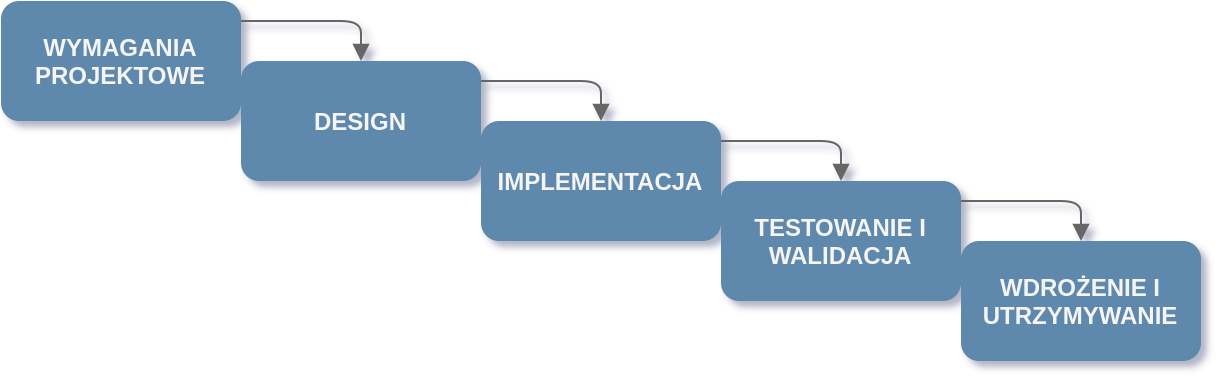
\includegraphics[scale=0.25]{waterfall_diagram.png}
    \newline
    Rys.1 - Cykl życia projektu w metodach kaskadowych
\end{center}

\subsubsection*{Wymagania projektowe}
Główna faza kontaktu z klientem. Analitycy zbierają wymagania od klienta i decydują, czy projekt zostanie zrealizowany. Szacowany jest jego czas trwania i koszt. Wynikiem końcowym tego etapu są często pierwsze dokumenty opisujące funkcjonalności w systemie - \textbf{Use cases - przypadki użycia} i \textbf{Dokument wizji projektu}

Dokument wizji projektu odpowiada na pytanie \textit{Jak będzie wyglądał projekt i jaką wartość dostarczy klientowi}. Zawierają się w nim między innymi cele projektu - jak rozwiązać \textit{problem} - czyli czego klient tak naprawdę potrzebuje, opisuje grupę odbiorców systemu, produkt końcowy i wartości które wniesie. Definiowany jest zakres systemu.

Przypadki użycia - use cases to szczegółowe opisy konkretnych funkcji w systemie opisane w formie ścieżek, jakie dany odbiorca będzie przechodził, żeby osiągnąć konkretny dla niego cel. Use cases są bardzo szczegółowe i przedstawiają wszystkie możliwe ścieżki i zachowania systemu.

Po tej fazie wszystkie Use Case'y dla projektu powinny zostać ukończone. Powstaje także \textbf{dokument wymagań projektowych} stanowiący bardziej techniczną i szczegółową wersję dokumentu wizji.

Przykładowy Use Case utworzony przeze mnie na potrzeby kursu z \textit{Inżynierii oprogramowania}:
\begin{tcolorbox}
    \subsubsection*{Kontekst: System zarządzania projektami w firmie produkującej filmy wideo}
    \subsubsection*{Use Case: Wprowadzenie projektu do systemu}
    \textbf{Aktor podstawowy: \textit{Szef firmy}}

    \subsubsection*{Główni odbiorcy i oczekiwania względem systemu}
    \begin{itemize}
        \item Szef: jest to podstawowa funkcja z jakiej szef będzie korzystał. Zależy mu na tym, aby dostęp do niej był szybki. Chce, aby wprowadzanie danych o projekcie było objęte pewnymi stałymi ramami, do których interfejs będzie dostosowany.
        \item Pracownik: oczekuje dostępu do nowego projektu wraz ze wszystkimi istotnymi informacjami o nim
        \item Klient: nie chciałby, aby musiał podawać dane kilkakrotnie, powinien mieć możliwość otrzymania informacji o stanie jego projektu
        \item Przedsiębiorstwo: potrzebuje dobrej organizacji wszystkich projektów, systematyzowania danych i ich bezpieczeństwa. W przypadku awarii systemu bądź sprzętu, musi mieć możliwość odzyskania krytycznych danych
    \end{itemize}

    \subsubsection*{Warunki wstępne}
    Szef jest zalogowany w systemie i ma dostęp do interfejsu zarządzania zadaniami. Baza danych ma wystarczającą ilość przestrzeni
    dyskowej, aby mógł zostać dodany wpis o projekcie.

    \subsubsection*{Warunki końcowe}
    Baza danych jest zaktualizowana o wpis z wszystkimi koniecznymi informacjami o projekcie. Ustalana
    jest data wprowadzenia projektu do systemu, generowany jest wpis w historii. Na osobnym dysku tworzona jest
    kopia zapasowa z wpisem do bazy. Projekt jest widoczny na tablicy pracowników i tablicy szefa. System jest w
    gotowości do przydzielenia ról i zadań pracownikom.

    \subsubsection*{Scenariusz główny}
    \begin{enumerate}
        \item Podczas rozmowy z klientem, szef otwiera moduł tworzenia projektu na swoim komputerze PC poprzez aplikacę webową
        \item Szef wprowadza dane o projekcie, wypełnia konieczne pola, między innymi: nazwę projektu, typ, krótki opis i zatwierdza utworzenie.
        \item Po zatwiedzeniu wyświetlane są wprowadzone dane w zwizualizowanej postaci (tabela)
        \item Szef ma możliwość modyfikacji lub zatwierdzenia projektu \newline \textit{W przypadku modyfikacji, powtarza krok 2 i 3}
        \item System przekazuje dane z klienta do serwera. Tworzony jest nowy wpis w bazie danych oraz kopia zapasowa.
        \item Na aplikacjach klienckich wyświetla się powiadomienie o nowym projekcie.
        \item Szef otrzymuje wiadomość zwrotną, że projekt został dodany pomyślnie
        \item W dowolnym momencie może zostać wprowadzana zmiana w danych projektu, mogą zostać załączone zewnętrzne dokumenty. \textit{Powtarzane są wtedy kroki 2-4}. Wpis w bazie danych oraz kopia zapasowa są aktualizowane.
    \end{enumerate}


    \subsubsection*{Rozszerzenia}

    \subsubsection*{* W dowolnym momencie system ulega awarii}
    Integralnośc danych musi zostać zachowana, zatem konieczna jest transakcyjność. Aktualizacje
    i tworzenie wpisów o projekcie musi zostać zaktualizowane tylko w przypadku kompletnego przesłania
    danych z aplikacji klienckiej do serwera i bazy danych
    \begin{enumerate}
        \item W przypadku automatycznego powrotu systemu do stanu gotowości, szef sprawdza, czy wpis o nowym projekcie został utworzony
              \begin{enumerate}
                  \item W przypadku braku wpisu, proces dodania projektu jest powtarzany
                  \item W przypadku poprawnego dodania wpisu, proces przebiega pomyślnie i szef może kontynuować pracę
              \end{enumerate}
        \item Gdy system nie powraca do stanu gotowości, szef musi poinformować administratora o błędzie w systemie. Administrator podejmuje odpowiednie kroki, aby przywrócić system do działania
    \end{enumerate}

    \subsubsection*{2. Niekompletne dane}
    W przypadku, gdy nie zostanie wprowadzona \textit{nazwa projektu}, projekt nie zostanie dodany, szef zostanie poinformowany o błędzie.

    \subsubsection*{5a. Błąd połączenia z serwerem lub błąd bazy danych}
    Wpis o nowym projekcie nie zostaje dodany. Aplikacja kliencka informuje o błędzie połączenia z serwerem i konieczności skontakowania się z administratorem


    \subsubsection*{5b. Projekt już istnieje}
    Gdy system bazodanowy wykryje, że projekt o tej samej nazwie istnieje już w bazie, wpis o nim nie jest dodawany. Interfejs sygnalizuje o błędzie i konieczności zmiany nazwy projektu.

    \subsubsection*{8a. Błędnie wprowadzone dane}
    Gdy system wykryje, że np. zmieniana jest nazwa projektu na nazwę już istniejącą, zwróci błąd.

    \subsubsection*{8b. Załączanie plików}
    Szef może chcieć dodać dokument do projektu.
    \begin{enumerate}
        \item Interfejs graficzny oferuję przesłanie i tym samym załączenie pliku do projektu.
        \item Szef wybiera plik i przesyła go na serwer.
              \begin{enumerate}
                  \item Obliczana jest ilość wolnego miejsca na dysku serwerowym. Gdy ilość wolnego miejsca nie jest wystarczająca do przesłania pliku, zostaje zwrócony błąd.
                  \item Podczas przesyłania występuje zerwanie połączenia. Plik nie jest przesłany i zostaje wysłane powiadomienie do aplikacji klienckiej.
                  \item Gdy plik jest wysłany poprawnie i znajduje się już na serwerze, tworzona jest jego kopia zapasowa, oraz dodawany jest wpis w bazie danych zawierający ścieżkę do dokumentu.
                  \item W przypadku sukcesu wszystkich procesów, zwracana jest wiadomość o sukcesie
              \end{enumerate}
    \end{enumerate}
\end{tcolorbox}
\subsubsection*{Design}
Na podstawie wcześniej zebranych wymagań analitycy we współpracy z architektami systemu decydują jak będzie wyglądał końcowy efekt i w jaki sposób zostanie utworzony. Podejmowane są tutaj takie decyzje jak wybór technologii i achitektura całego systemu, tworzone są wstępne projekty intefrejsu. Definiowany jest zakres systemu, wymagania funkcjonalne i niefunkcjonalne czy kryteria akceptacji i ryzyka projektowe.

\subsubsection*{Implementacja}
Zespół programistów ze współpracy z architektami systemu implementują jego design. W tej fazie powinna powstać większość bytów programistycznych realizująca cały zakres systemu.

\subsubsection*{Testowanie i walidacja}
Po ukończeniu prac programistycznych zespół odpowiedzialny za testowanie systemu rozpoczyna swoją pracę i sprawdza, czy cały system działa. Implementacja jest weryfikowana pod kątem spełnienia wymagań projektowych, tworzone są raporty z testów, ostatnie funkcjonalności są zaimlpementowane. Wszystkie use casy są zrealizowane.

\subsubsection*{Wdrożenie i utrzymanie}
System jest przygotowywany do oddania klientowi. Administratorzy systemowi wdrażają cały projekt według zaplanowanego rozwiązania architektonicznego. Tworzone są dokumenty instruujące jego odbiorców jak go używać.

Po wdrożeniu system jest dalej utrzymywany według wcześniej ustalonych zasad, poprawiane są błędy, które wcześniej nie zostały wykryte. System nie powinien być już dalej uzupełniany o nowe funkcjonalności.

\subsection{Agile}
Agile to rodzina metod, która zaczęła rozwijać się na przestrzeni lat 80-tych i 90-tych ubiegłego stulecia jako opozycja starego podejścia metodyk kaskadowych\cite{scrum}, jako, w pewnym sensie, nauka na błędach. Deweloperzy byli zmęczeni wielkimi korporacyjnymi strukturami stojącymi za kaskadowym procesem, które tłumiły wszelkie indywidualne inicjatywy na rzecz "decyzji z góry". Kreatywność nie była cechą cenioną. Programiści nie musieli myśleć - ich zadaniem było realizowanie architektury zaplanowanej przez architekta. Nikt nie zastanawiał się nad tym, czy zadania im powierzone mają sens.

Mimo wszystko Agile nie miał siły przebicia i przez wielu uważany był za żart. Dopiero na początku ówczesnego tysiąclecia Agile zaczynał zyskiwać na popularności, natomiast w praktyce zaczął być stosowany dopiero w okolicach roku 2010.

Agile jest w pewnym sensie procesem odwrotnym do metodyk kaskadowych\cite{scrum} Kaskada, czyli jeden etap po drugim - w Agile wszystkie etapy dzieją się tak naprawdę jednocześnie. Stały schemat metody pracy i brak reakcji na błędy został zastąpiony ciągłymi zmianami i budowaniem procesu w oparciu o niepowodzenia. Ba, zmiany stały się nieodłączną częścią całego procesu. Kontakt z klientem jest bardzo częsty i aktywny przez cały. Indywidualne inicjatywy członków zespołu budują cały proces. Nowe funkcjonalności systemu są testowane na bieżąco. Metodologie Agile idealnie podsumowuje \textbf{Manifest Agile (Agile Manifesto)}

\subsubsection{Manifest Agile}

\begin{center}
    Ludzie i interakcje ponad procesami i narzędziami

    Działające produkty ponad złożoną dokumentacją

    Współpraca z klientem ponad negocjacją kontraktu

    Reagowanie na zmiany ponad trzymaniem się planu\cite{scrum}
\end{center}

\subsubsection*{Ludzie i interakcje ponad procesami i narzędziami}
Największy wpływ na rozwój projektu mają właśnie ludzie - to dzięki ich kreatywności i zaangażowaniu skomplikowana maszyna projektowa idzie do przodu. Narzucanie ścisłych zasad procesowych ogranicza możliwości zespołu, a skomplikowane narzędzia wcale nie ułatwiają im pracy.

\subsubsection*{Działające produkty ponad złożoną dokumentacją}
Tutaj mowa o wspomnianym wcześniej podejściu odwrotnym do kaskadowego - wytwarzając skomplikowane oprogramowanie jako jedną całość tracimy możliwość wprowadzania zmian w trakcie projektu - Agile mówi, żeby poszczególne etapy projektu były małe i kończyły się jakąś działającą częścią systemu. Dzięki temu możemy raportować klientowi postępy pracy i łatwo dostosowywać się do jego uwag czy sugestii. Inkrementacyjne wytwarzanie oprogramowania umożliwia też stałe testowanie i bardziej realistyczne określanie dalszych ryzyk w projekcie.

\subsubsection*{Współpraca z klientem ponad negocjacją kontraktu}
W modelu kaskadowym wkład w projekt klienta był tak naprawdę znikomy. Na początku projektu podczas zbierania wymagań decydowano tak naprawdę czy projekt ma sens, czy nie. Zespół obawiał się wszelkich zmian ze strony klienta po zatwierdzeniu wymagań. W Agile klient jest stale zaangażowany w rozwój projektu. Wymagania zawsze mogą ulegać zmianie i iteracyjny rozwój oprogramowania jest na nie otwarty. Satysfakcja klienta również jest dużo wyższa, stałe postępy w pracy nad projektem są dla niego widoczne.

\subsubsection*{Reagowanie na zmiany ponad trzymaniem się planu}
Nie pracowałem nigdy w projekcie, w którym wszystko wychodziłoby tak, jak zostało to na początku zaplanowane. W Agile zespół powinien być stale otwarty na pojawiające się zmiany i dostosowywać swoje zmiany pracując razem z nimi.

\paragraph{}
Metody kaskadowe były określane jako "powtarzalne"\cite{scrum}, bo każdy projekt realizowany był w bardzo podobny sposób. W Agile można zaobserwować "odwrotne" podejście - każdy projekt należy traktować w inny sposób. Specyfika każdego projektu może decydować o tym jak będzie wyglądała praca zespołu. Sam zespół składa się z ludzi, których zachowania i charaktery wcale nie są powtarzalne, jak to zakładało podejście kaskadowe. Każdy projekt realizowany zwinnie ma w pewnym sensie swojego własnego Agile'a, stale rozwijanego jako reakcja na zmiany i problemy. Zespół "doskonali" proces na przestrzeni jego rozwoju.

\subsubsection{Cykl życia projektu}
Cykl życia projektu w metodykach zwinnych można określić hasłem "iteracyjny". Każda iteracja rozpoczyna się określeniem zakresu pracy i kończy gotową, działającą częścią systemu przybliżającą projekt do osiągnięcia większych celów, implementacyjnych i biznesowych. Ilość takich iteracji w projektach zależy od czasu trwania jednej iteracji i całego zakresu systemu.

W kaskadowym schemacie każdy z etapów obejmował całośc sytemu. Wymagania, projekt, implementacja, testy i wdrażanie. W zwinnych metodykach wszystkie te fazy dotyczą jednej iteracji i często wykonywane są asynchronicznie.

\begin{center}
    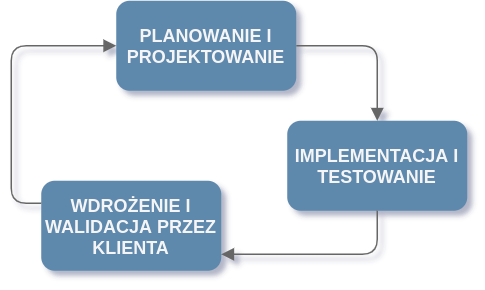
\includegraphics[scale=0.35]{agile.png}
    \newline
    Rys. 2 - Cykl życia projektu w metodach zwinnych
\end{center}

Ryzyka projektowe są stale ewaluowane podczas każdej iteracji. Agile wprowadziło też ideę \textit{Proof of concept} - działający prototyp, który pozwala na dokładne badanie ryzyka wynikającego z proponowanych rozwiązań. Takie prototypy mogą być tworzone w dowolnym momencie pomiędzy iteracjami i to zespół decyduje, kiedy stworzenie \textit{PoC}\footnote{Skrót od Proof of concept} wprowadzi korzyści dla projektu.

Prototypy wcale nie muszą kończyć się powodzeniem - porażka może stanowić dla zespołu pewien rodzaj komunikatu, że wybrane przez nich rozwiązanie jest zbyt ryzykowne i zdecydować się na inne. \textit{PoC} często są do użytku wnętrznego, natomiast nic nie stoi na przeszkodzie prezentacja wyników klientowi - mogą one stanowić dowód trudności rozwiązań przez niego proponowanych i rozpozcąć dyskusję nad zmianą takich wymagań.

\subsubsection*{Zbieranie wymagań - User Stories jako nowe przypadki użycia}
Przypadki użycia z modelu kaskadowego były bardzo obszerne i mimo swojej złożoności czasami wcale nie dawały jawnego obrazu na to, jakie oczekiwania wobec niego mają odbiorcy. Informacje w nim przekazywane były zupełnie surowe - deweloperzy nie mieli okazji postawić się w roli użytkownika systemu, a analitycy spędzali większość czasu na budowaniu takich use case'ów, które pokryją dokładnie każdy scenariusz zachowania projektowanego systemu.

Zgodnie z hasłem "Działające produkty ponad złożoną dokumentacją" Agile zaproponowało alternatywny sposób zbierania wymagań - \textbf{User Stories}.

Zamiast długich przypadków użycia, User Stories mają być krótkie; ich forma wygląda następująco:

\begin{center}
    \textit{Jako \textbf{aktor}, chcę \textbf{wykonać czynność}, aby \textbf{osiągnąć pewien cel}.}
\end{center}

W odróżnieniu od przypadków użycia, które tworzone były przez analityków nie będącymi użytkownikami systemu, User Stories są tworzone we współpracy z klientem czy aktorami w systemie - ich prostota na to pozwala.

User stories stanowią najmniejszą jednostkę pracy dla zespołu.

\paragraph{Przykłady User Stories:}

\begin{center}
    Jako Pracownik che móc generować raporty, aby zwizualizować swoim klientom, szefowi lub kolegom z zespołu postępy, bądź informacje o postępach nad projektem.

    \paragraph{}
    Jako Użytkownik chce mieć możliwość zmiany danych osobowych w systemie na wypadek przeprowadzki, lub zmiany ważnych danych.

    \paragraph{}
    Jako Administrator potrzebuje funkcji zalogowania się jako inny użytkownik w systemie, aby diagnozować konkretne problemy napotkane przez tego użytkownika.

    \paragraph{}
    Jako Użytkownik chce móc edytować wysłane wiadomości na wypadek pomyłkek, literówek, żeby utrzymać jakość swoich wypowiedzi na wysokim poziomie

\end{center}

Ilość zrealizowanych User Stories na danym etapie projektu stanowi dobrą metrykę faktycznych postępów nad systemem. Reprezentują mierzalną wartość dla klienta, który podczas iteracji jest w stanie oceniać, czy są zrealizowane poprawnie.

\section{Wybrane metodyki zwinne}

\subsection{Scrum}

Scrum sam w sobie nie jest tak naprawdę metotyką, a bardziej \textit{frameworkiem}\footnote{z ang. szkielet, struktura, model} opisujący pewne praktyki opisujące jak budować taki proces\cite{scrum}. Znamy zasady gry, ale sposób na jej zwycięstwo zależy już od nas, czy w przypadku projektów informatycznych, od naszego zespołu. Scrum to zatem w pewnym sensie metoda działania.

\subsubsection{Role w zespole}

\subsubsection*{Product Owner - właściciel produktu}
\textit{Właściwiel produktu}, jak sama nazwa wskazuje, odpowiada za produkt tworzony przez zespół. Jego głównymi zadanami jest dbanie o \textit{Product backlog} i o wartość pracy zespołu.

W odróżnieniu od metod kaskadowych, gdzie rola \textit{manedżera projektu} czy \textit{analityka} była rozłączna od całego zespołu, tutaj Product Owner jest jego częścią. "Opiekuje" się produktem tworzonym przez zespół. Wymagania nie są już tworzone tylko przez klienta i spisywane przez analityków, zespół tworzy je razem z Product Ownerem\cite{scrum}.
\subsubsection*{Scrum Master}

\textit{Scrum Master} jest pewnego rodzaju strażnikiem całego zespołu Scrumowego. Dba on o to, aby zespół mógł pracować bez żadnych zakłóceń zewnętrznych, takich jak ingerencja wyższych kierowników, czy problemy firmy. Jest też swojego rodzaju strażnikiem procesu, ale rozumianym w mniej restrykcyjny sposób - dba o to, żeby wszyscy członkowie zespołu rozumieli tą metodykę i poprawnie ją stosowali. Wspomaga jego rozwój, dba o relacje między członkami zespołu. Asystuje Product Owner'a w kwestiach produktowych. Sam Scrum Master nie powinien uczestniczyć w programistycznych dyskusjach\cite{scrum}.

\subsubsection*{Deweloper, czyli "zwykły" członek zespołu}
Członkowie zespołu Scrumowego to nie koniecznie tylko programiści. W zależności od tego, czego potrzebuje zespół do realizowania User Stories mogą się w nim znaleźć takie role jak grafik, tester, projektant interfejsu, czy nawet tłumacz, jeżeli produkt tego wymaga. Ich rolą jest realizowanie User Storiesów. W odróżnieniu od programistów czy testerów w kaskadowym podejściu, zespół uczestniczy w spotkaniach produktowych i jest w stanie wpłynąć na to, jak wyglądają wymagania projektowe. Zespół jest samoorganizacyjny, to jego członkowie decydują o tym, w jaki sposób wykonują zadania podczas Sprintu.

\subsubsection{Organizacja pracy}

\subsubsection*{Agilowy cykl życia projektu w Scrumie}

\begin{center}
    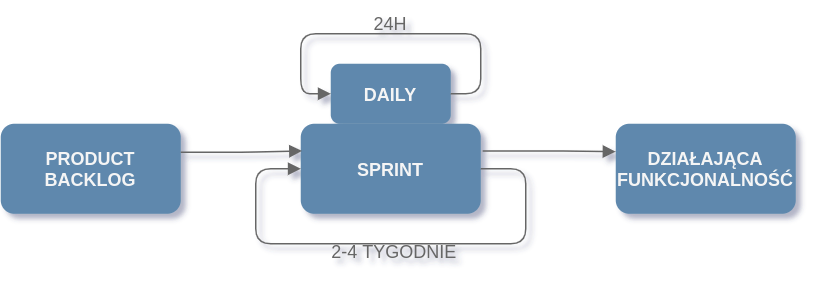
\includegraphics[scale=0.35]{scrum.png}
    \newline
    Rys. 3 - Sprint w Scrumie
\end{center}

\subsubsection*{Product Backlog}
Product Backlog \textit{z ang. Rejestr Produktu} przechowuje wymagania projektowe od klienta. Zawierają się w nim głównie User Stories, pogrupowane w większe fragmenty zwane \textbf{Epicami} stanowiące pewne kamienie milowe dla projektu.

\subsubsection*{Daily}
Daily to inaczej codzienne spotkanie w Scrumie. Jego głównym celem jest przedstawienie obecnego stanu realizowanych zadań przez członków zespołu. Codzienne spotkania mają charakter wewnętrzny. Zespół opowiada o postępach nad zadaniami, sygnalizuje problemy i przeprowadza krótkie dyskusję na temat wykonywanych prac.

Takie spotkania informują cały zespół o tym, co się dzieje w projekcie. Członkowie mają informację o zadaniach, które nie są przez nich realizowane, co daje im szeroki punkt widzenia na cały projekt. Mogą komentować poczynania innych, sugerować alternatywne rozwiązania.

\subsubsection*{Sprint}
Sprint, czyli według Agilowego słownika, iteracja w projekcie, stanowi główny rdzeń całego procesu. Wszystkie najważniejsze założenia Scruma są realizowane właśnie w jego obszarze.

Sprint rozpoczyna się tzw. \textit{Sprint planningiem}, czyli planowaniem sprintu.

\subsubsection*{Sprint Planning}

Celem planowania jest wybranie realizowanych User Stories i rozbicie ich na zadania, często mające formę programistyczną.

Wybór realizowanych Stories jest kluczową rzeczą dla rozpoznawania ryzyka w projekcie i priorytetyzacji. Zespół razem z \textit{Product ownerem} skupia się nad tym, co chce w danym sprincie osiągnąć\cite{scrum}.

Przy wyborze User Stories zespół szacuje, ile jednostek czasu jest w stanie na nie poświęcić, na przykład na podstawie metryk z wcześniejszych sprintów\cite{scrum}.

User Stories są rozbijane na mniejsze zadania, którym przypisywane są jednostki czasowe przewidziane na ich realizacje. Takie zadania mają na celu pomóc zespołowi w rozdzieleniu pracy między członków.

\subsubsection*{Praca podczas Sprintu}
Po Sprint Planningu zespół skupia się na realizowaniu zadań. Codziennie odbywają się Daily.

Organizacja pracy zależy tutaj tylko i wyłącznie od zespołu - w zasadach Scruma nie jest to zawarte - tu można zaobserwować wykorzystanie jednego z założeń Agile - \textit{Ludzie i interakcje ponad procesami i narzędziami}. To zespół decyduje w jaki sposób realizuje zadania.

\subsubsection*{Definiton of done}
Definition of done \textit{z ang. miara kompletności} to abstrakcyjne pojęcie, które definiowane jest w każdym projekcie w inny sposób. Mówi ono o tym, jakie kryteria powinno spełniać zadanie czy User Story, żeby było określone jako ukończone. Ciężko jest podać dokładną definicję takiego abstrakcyjnego pojęcia.

Przykłady \textit{definition of done}:
\begin{center}
    \textit{Każde zadanie programistyczne powinno być odpowiednio przetestowane testami integracyjnymi, jednostkowymi i manualnymi.}

    \textit{Przy wprowadzaniu skomplikowanych zmian do systemu powinna zostać utworzona krótka dokumentacja opisująca sposób działania nowych rozwiązań.}

    \textit{Zadania powinny być uznane za ukończone tylko wtedy, jeżeli wprowadzone w ramach nich zmiany będą dostępne dla klienta na serwerze produkcyjnym.}
\end{center}

\subsubsection*{Retrospektywa}
Sprint nie narzuca zasad pracy podczas Sprintu i to zespół decyduje o jego dokładnym przebiegu. Retrospektywa to spotkanie mające na celu usprawniać działanie zespołu podczas trwania Sprintu. Takie spotkanie powinno odbywać się jeden raz w ciągu Sprintu.

Na retrospektywie każdy z członków zespołu może powiedzieć co jego zdaniem udało się zrobić dobrze, a co nie, oraz zasugerować rozwiązania danych problemów.

Rezultatem retrospektywy są \textit{Action Points} \textit{(z ang. punkty akcji)}, czyli konkretne działania bądź zmiany w procesie jakie zespół zastosuje podczas następnych sprintów, utworzone na podstawie odbytych dyskusji.

\subsection{Kanban}
Metodyka ta została stworzona przez Taiichiego Ohno pracującego w japońskiej firmie *Toyota*\cite{kanban}.Kanban w odóżnieniu od Scruma charakteryzuje się ciągłym przepływem zadań (określanym mianem \textit{karteczek}) / User Stories i nie definiuje żadnych ról. Jego głównym celem jest wizualizacja pracy projektowej w zespole. Kanban to "lekka" metodyka, w czystej postaci znajdująca swoje zastosowanie głównie w niewielkich projektach i zespołach\cite{kanban2}.

\subsubsection{Przepływ zadań}

\begin{center}
    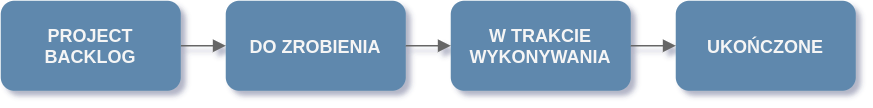
\includegraphics[scale=0.35]{kanban.png}
    \newline
    Rys. 4 - Przepływ zadań w Kanbanie
\end{center}

Zadania w tablicy Kanbanowej przepływają od lewej kolumny do prawej przy zmianie ich statusu. Głównym założeniem jest zredukowanie ilości zadań w danej kolumnie. "Karteczka" nie powinna znajdować się w jednej kategorii zbyt długo.

\subsubsection*{Project Backlog}
Podobnie jak w Scrumie, User Stories utworzone na podstawie wymagań projektowych znajdują się w Project Backlogu. W tamtej metodyce wybieranie zadań z Backlogu było skomplikowane i wymagało podejmowania świadomych decyzji, które wpływały na dalszy rozwój projektu. W Kanbanie to zespół na bieżąco decyduje o tym, jakie zadania z Backloga będą realizowane w danej chwili.

\subsubsection*{Skalowalność tablicy Kanbanowej}
Poza wyróżnionymi głównymi kolumnami wyróżnionymi powyżej, tablicę można dowolnie rozszerzać o nowe kolumny i wiersze. Jeżeli w zespole znajdują się dedykowani testerzy i produkt tego wymaga, możemy dodać nową kolumnę jako następną po "W trakcie wykonywania" i nazwać ją "Testowanie". Testerzy będą zajmowali się zadaniami, które oczekują na testy właśnie z tej kolumny.

Dodawanie kolejnych etapów dla stopnia ukończenia zadania będzie skutkowało rozwojem tablicy o kolejne kolumny. Możemy również stworzyć nowy wiersz (często określany jako \textit{swim lane}), w którym zadania będą przechodzić tą samą ściężkę, ale mogą być wyróżnione ze względu na priorytet, lub kategorię.

\subsection{Scrumban}
W Scrumie organizacja pracy podczas Sprintu nie była ustalona - to zespół decydował w jaki sposób przechodzi przez cały Sprint. Implementacja Kanbana do organizacji zadań stała się bardzo popularnym rozwiązaniem w implementacjach Scruma i zyskała tytuł \textit{Scrumban}


\section{Proces w WMI Adventure}
WMI Adventure od samego początku nie miał być projektem komercyjnym. Dostępność członków zespołu nie pozwalała na stosowanie na przykład czystej metodyki Scrum. Codziennie spotkania (daily) nie wnosiłyby niczego dla zespołu - często zdarzałyby się sytuacje, gdzie zespół nic nie zrobił przez ostatnie 24 godziny.

Dodatkowo specyfika projektu nie definiuje konkretnego klienta. WMI Adventure to gra przeznaczona dla wąskiej społeczności wydziału wywodząca się z naszego własnego pomysłu. Współpraca z potencjalnymi użytkownikami systemu wyglądała w zupełnie inny sposób, gdyż to my proponowaliśmy produkt i jego specyfikację licząc jedynie na opinię klientów.

\subsection{Metodyka}
Scrumban był metodyką najbardziej zbliżoną do naszych potrzeb i własnie na niego padł wybór. Nie podążaliśmy ściśle za proponowanymi zasadami - wykorzystaliśmy zwinne podejście także do samej metodyki modyfikując ją z każdą kolejną iteracją.

Pierwszą wprowadzoną zmianą już w pierwszym sprincie to daily co drugi dzień. Wspominałem już o ograniczonej dostępności czasowej członków zespołu, stąd ta decyzja. Zespół doszedł do wniosku, że robiąc takie daily codziennie tracilibyśmy czas, który moglibyśmy poświęcić na pracę indywidualną.

Taka wersja metodyki zapewniła nam dobry balans między czasem poświęconym na proces a pracą nad funkcjonalnościami w projekcie. Dołącznie do Scruma tablicy Kanbanowej zapewniło nam też organizację mniejszych zadań wewnątrz każdego sprintu.

\subsection{Role w zespole}
Zespół liczył zaledwie 4 członków, więc nie byliśmy w stanie rozdzielić całkowicie ról deweloperów i tych wyróżnionych przez Scrum. Scrum Master i Product Owner pełnili zatem też role programistyczne.

\begin{itemize}
    \item \textbf{Mateusz Tylka} - Product Owner, deweloper - frontend
    \item \textbf{Dawid Korybalski} - deweloper - frontend
    \item \textbf{Michał Czekański} - deweloper, DevOps - backend
    \item \textbf{Marcin Kostrzewski} - Scrum Master, deweloper, DevOps - backend i UI/UX
\end{itemize}

Można zauważyć, że w zespole można wyróżnić dwa mniejsze dwuosobowe zespoły podzielone ze względu na zakres prac programistycznych; tj. zespół backendowy i frontendowy. Podział ten był jednak jedynie symboliczny - zespół pracował zawsze razem, realizując te same cele realizując zadania z tej samej tablicy. Dwie siły były wyróżnione ze względu na naszye kompetencje i podział był naturalny.

Podczas trwania całego projektu role te coraz bardziej się zacierały. Role backendowe i frontendowe przekształcały się na bardziej wszechstronne i zaangażowanie w produkt i proces rozmyło rolę Product Ownera i Scrum Mastera na wszystkich członków zespołu.

Od października, czyli mniej więcej w połowie trwania projektu zespół zmniejszył się do trzech członków i skład od tego czasu prezentował się następująco:
\begin{itemize}
    \item \textbf{Mateusz Tylka} - Product Owner, deweloper - frontend i UI/UX
    \item \textbf{Michał Czekański} - deweloper, DevOps - fullstack i UI/UX
    \item \textbf{Marcin Kostrzewski} - Scrum Master, deweloper, DevOps - fullstack i UI/UX
\end{itemize}

\subsection{User Stories}
\begin{tcolorbox}
    W każdym story pomijamy aktora, jest napisane w nagłówku kto nim jest. Dodatkowo historie podzielone są na sekcję będące częściami systemu.

    \begin{enumerate}
        \item Użytkownik: \textbf{Student}
              \begin{enumerate}
                  \item Tryb Battle
                        \begin{enumerate}
                            \item Chcę w głównym widoku wejść w Tryb Battle i zobaczyć listę graczy, których mogę wyzwać na pojedynek oraz tych których nie mogę i chce wiedzieć dlaczego nie mogę.
                            \item Chcę mieć możliwość wyboru przeciwnika, aby mieć kontrolę nad tym, z kim będę walczył.
                            \item Po przejściu w Tryb Battle chcę móc wyszukać użytkowników po nazwie, aby stoczyć pojedynek z konkretnym studentem.
                            \item Oprócz wyszukiwania przeciwników, chcę aby aplikacja pokazała mi kilku sugerowanych użytkowników do walki, abym nie musiał za każdym razem wyszukiwać konkretnych graczy.
                            \item Po wyborze przeciwnika chciałbym zobaczyć jego profil, żeby móc przygotować się do walki.
                            \item W widoku profilu przeciwnika chciałbym dowiedzieć się o jego procencie wygranych, punktach zdobytych w aplikacji, pozycji w rankingach, aktualnym semestrze, żeby móc ocenić swoje szanse na wygraną.
                            \item Po wyborze przeciwnika chcę mieć możliwość powrotu i wyboru innego przeciwnika, aby uniknąć nieprzemyślanych decyzji i ewentualnych missclicków.
                            \item Chcę widzieć przebieg walki, żeby czerpać z niej satysfakcję i zobaczyć jak działają moje karty.
                            \item Przed rozpoczęciem i w trakcie walki chcę mieć możliwość fast-forwardu, czyli automatycznego rozegrania pojedynku bez wizualizacji, żeby szybko dowiedzieć się o jej wyniku i nie tracić czasu.
                            \item Po wygranej lub przegranej walce chcę zobaczyć skutki pojedynku, żeby wiedzieć co się stało i ile zdobyłem/straciłem punktów.
                            \item Chcę, aby przebieg walki, czyli między innymi karty moje i przeciwnika, został zapisany. Chcę móc mieć dostęp do kilku ostatnich historycznych pojedynków, żeby ocenić dobór swoich kart i przygotować się lepiej do przyszłych walk.
                            \item Nie chcę, żeby jeden przeciwnik atakował mnie cały czas znając moją talię, aby uniknąć masowych strat punktów.
                            \item Przed każdą walką chcę mieć dodatkowo możliwość łatwego przejścia do mojej talii kart, aby dostosować ją do konkretnej walki bez konieczności powrotów do poprzednich menu.
                            \item Po przejściu w Tryb Battle w pierwszym widoku chcę zobaczyć moje statystyki z tego trybu, takie jak punkty, stoczone walki, wygrane walki razem z procentem wygranych, aby po każdej walce widzieć, jak zmienia się moja pozycja w rankingu bez potrzeby przechodzenia do innych widoków.
                            \item Po przejściu w Tryb Battle w pierwszym widoku chcę zobaczyć moją talię oraz mieć możliwość przejścia do zmiany talii, by móc zweryfikować jej skład i ewentualnie zmienić ją przed pojedynkami.
                            \item Po skończonej walce chcę mieć możliwość powrotu do Trybu Battle, żeby nie musieć przeklikiwać przez całą aplikację.
                            \item Chcę aby system walki kartami był zbalansowany i atraktyjny, żebym cieszył się z gry i nie czuł, że wygrywanie jest zbyt łatwe, lub zbyt trudne posiadając daną ilość kart i bedąc na X semestrze.
                            \item Chcę żeby tylko osoby o podobnym poziomie bitewnym co mój mogły mnie wyzywać na pojedynki, abym nie mógł łatwo wygrywać ciągle z tą samą osobą, lub jakaś mocniejsza osoba nie mogła w kółko nabijać sobie na mnie punktów.
                            \item Chcę aby konkretne karty były atrakcyjne, miały informatyczny przekaz i sensowne działanie, żeby cieszyć się z pojedynkowania, układania talii oraz kolekcjonowania kart.
                            \item Chcę, aby było jaśnie określone, czy karty mogą mi się przydać do czegoś więcej niż tylko do Trybu Battle i mieć jasny przekaz do czego jeszcze mogę ich użyć lub jakie dają korzyści, żeby wiedzieć co mogę z nimi zrobić i cieszyć się z aplikacji.
                        \end{enumerate}
                  \item Tryb Adventure
                        \begin{enumerate}
                            \item Chcę w głównym widoku wejść w Tryb Adventure i zobaczyć wszystkie historie wyróżnione na te dostępne do przejścia, te które przeszedłem i te które nie są jeszcze dostępne.
                            \item Chcę móc "przyśpieszyć" wyświetlanie napisów dialogowych, bo mogę czytać je szybciej i nie chcę tracić niepotrzebnie czasu.
                            \item Chcę mieć możliwość powrotu do historii, które już przeszedłem, aby jeszcze raz je sobie przypomnieć.
                            \item W dowolnym momencie chcę móc wyjść z trybu, żeby móc skupić się na innej rzeczy, którą w danej chwili chcę zrobić.
                            \item Po wyjściu z historii chcę mieć możliwość powrotu do konkretnego momentu, w którym skończyłem, żeby nie musieć oglądać dwa razy tego samego.
                            \item Jeżeli zdobędę nową kartę, chcę być o tym wyraźnie powiadomionym, zobaczyć czym ta karta jest, żeby dowiedzieć się, że w mojej talii pojawiła się nowa bez konieczności wychodzenia z trybu.
                            \item Chcę wyraźnie widzieć, która postać mówi aktualny dialog, żeby nie gubić się w treści.
                            \item Chcę cały czas widzieć pasek postępu w historii, którą przechodzę, żeby móc ocenić ilość czasu jaką muszę poświęcić na ukończenie jej.
                            \item Chcę mieć możliwość pokonywania kluczowych postaci w Trybie Adventure, żeby czerpać satysfakcję z progresowania w aplikacji.
                            \item Przed walką z bossem chcę mieć możliwość zmiany mojej talii, żeby nie musieć wychodzić z Trybu Adventure w celu dostosowania mojej talii pod bossa.
                            \item Po skończonej walce z bossem nie chcę być wyrzucany z Trybu Adventure, żeby móc dalej kontynuować historię.
                            \item Jeżeli pokonanie bossa wiążę się ze zdobyciem nowej karty, to przed walką chcę się o tym dowiedzieć, żeby mieć większą chęć do walki.
                        \end{enumerate}
                  \item Rankingi
                        \begin{enumerate}
                            \item Chcę mieć możliwość wyboru kategorii rankingowych, żeby w jednym momencie widzieć tylko tą, która mnie interesuje.
                            \item Chcę, żeby kilku najlepszych graczy było wyraźnie zaznaczonych, aby czerpać większą satysfakcję jeżeli to ja będę wśród nich.
                            \item Przy każdym użytkowniku w rankingu chcę widzieć jego pozycję i wynik, aby łatwo odczytać informację o nich.
                            \item Chcę móc kliknąć na dowolnego użytkownika żeby wyświetlić jego profil w celu pozyskania informacji o nim.
                            \item Po wyświetleniu wybranego profilu chcę mieć możliwość stoczenia z nim pojedynku, żeby nie musieć zapamiętywać jego nazwy do późniejszego wyszukiwania w Trybie Battle.
                            \item Chcę wyszukiwać użytkowników po nazwie, żeby zobaczyć ich pozycję w rankingu, ich profil.
                            \item Chcę zawsze widzieć swoją pozycję i wynik w kategorii, którą aktualnie wyświetlam, żeby mieć do niej łatwy dostęp i nie musieć przechodzi do swojego profilu.
                        \end{enumerate}
                  \item Profil użytkownika
                        \begin{enumerate}
                            \item Chcę widzieć swoją nazwę i statystyki, żeby analizować swoje postępy w aplikacji.
                            \item Chcę móc łatwo edytować swoją talię kart, żeby próbować różne kombinację bez konieczności wchodzenia w tryb Battle.
                            \item Przy dostosowaniu talii chcę widzieć wszystkie dostępne karty, aby mieć możliwość łatwej zmiany talii.
                            \item Chcę zobaczyć informację o karcie którą wybiorę, żeby dowiedzieć się co ona robi i zdecydować czy chcę coś z nią zrobić.
                            \item Chcę mieć wgląd na wszystkie karty jakie posiadam, żeby cieszyć się swoją kolekcją.
                            \item W edytorze talii chcę, aby nowo zdobyte karty były jakoś oznaczone, aby nie musieć ich wyszukiwać wśród wszystkich innych.
                            \item Chcę widzieć poziomy swoich kart, żeby łatwiej dostosowywać talię.
                            \item Chcę zawsze widzieć ilość punktów Skilli, żeby łatwiej podejmować decyzję ulepszania kart.
                            \item W każdej chwili chcę mieć możliwość podjęcia się rozwiązania quizu, żeby otrzymać nowe punkty Skilli.
                            \item Chcę mieć dostępne dwie talie kart - do obrony i do ataku, aby odpowiednio przygotować się na nadchodzące pojedynki
                        \end{enumerate}
                  \item Quizy
                        \begin{enumerate}
                            \item Chcę mieć dostęp do widoku ze wszystkimi pytaniami podzielone na kategorie, na które do tej pory udzieliłem poprawnej odpowiedzi w quizach, aby móc je sobie przypomnieć.
                        \end{enumerate}
                  \item Pozostałe
                        \begin{enumerate}
                            \item  Chcę mieć możliwość wyłączenia efektów dźwiękowych w aplikacji, aby nie musieć ich słyszeć gdy tego nie potrzebuję.
                            \item Chcę mieć możliwość zgłoszenia błędu w treściach aplikacji, żeby dać informację zwrotną twórcom, aby poprawili błąd.
                            \item Po wejściu do aplikacji chcę dowiedzieć się, czy trwa obecnie event losowy, aby zdobywać nowe karty, punkty PU i utrzymywać codzienną aktywność w grze.
                            \item Jeżeli nie mogę dołączyć do eventu losowego, chcę znać powód, aby dostosować się do jego wymagań i wziąć w nim udział.
                            \item Chcę dostawać powiadomienia informujące mnie o nowej zawartości w aplikacji, żebym mógł ją sprawdzić.
                            \item Chcę, aby opis do czego służy ta aplikacja i co można w niej robić nie był zbyt długi i znajdował się na jej stronie głównej bez potrzeby rejestracji, ani logowania, żeby łatwo się dowiedzieć, czy będę zainteresowany używaniem tej aplikacji.
                        \end{enumerate}
              \end{enumerate}
        \item Użytkownik: \textbf{Twórca}
              \begin{enumerate}
                  \item Kreator Historii
                        \begin{enumerate}
                            \item Chcę móc dodawać swoje obrazy, aby potem wykorzystać je w historiach.
                            \item Chcę obsługę przezroczystości, żeby postacie dobrze wyświetlały się na tłach.
                            \item Chcę mieć możliwość symulacji historii, żeby zobaczyć jak będzie wyświetlana użytkownikom i poprawić ewentualne błędy.
                            \item Chcę móc dostosować parametry historii, aby wyświetlały się konkretnym studentom na danym semestrze z danym przedmiotem.
                            \item Chcę dodawać wiele emocji dla postaci i móc je wywoływać w konkretnych dialogach, aby tworzyć bardziej dynamiczne historie.
                            \item Chcę ustawić kiedy i jaką kartę użytkownik zdobędzie, żeby tworzyć historię, po których użytkownik zdobywa nowe karty.
                            \item Chcę móc wywoływać proste animacje, żeby historie lepiej wyglądały.
                            \item Chcę móc usuwać swoje dodane obrazy jeśli jednak zdecyduje się na inny wygląd sceny, aby historia była zaprezentowana według mojej wizji.
                            \item Chcę dostać powiadomienie czy wysłana przeze mnie historia została wysłana pomyślnie, aby wysłać ją jeszcze raz w razie potrzeby.
                            \item Chcę móc wybierać i usuwać grafiki już znajdujące się w bazie danych aplikacji aby je wykorzystywać do swojej historii.
                        \end{enumerate}
                  \item Kreator Kart
                        \begin{enumerate}
                            \item Chcę móc dodawać swoje obrazy, aby tworzyć unikalne karty.
                            \item Chcę wybierać efekty z listy, żeby tworzyć dynamiczne karty.
                            \item Chce móc dostosować parametry karty, żeby miały konkretne efekty w trybie Battle.
                            \item Chcę zdecydować w jaki sposób karta będzie ulepszana przez punkty Skilli.
                            \item Chcę móc tworzyć karty wszelkiego rodzaju, aby przyczynić się do rozwoju treści w aplikacji.
                            \item Chcę, aby karta zawierała tytuł, przedmiot i krótki opis, aby móc charakteryzować karty i dzielić je na kategorie.
                            \item Chcę móc nadać karcie więcej niż jeden efekt, aby karty były bardziej różnorodne.
                            \item Chcę mieć możliwość tworzenia kart dających mocne benefity, ale też pewne kary dla posiadacza, żeby karty były urozmaicone.
                            \item Chcę tworzyć karty, które na różnych poziomach będą miały różne efekty, żeby same karty i ich ulepszanie na wyższe poziomy było ciekawsze.
                            \item Chcę mieć możliwość dołączenia dodatkowych uwag w formie tekstowej do mojego zgłoszenia nowej karty, żeby przekazać administratorom informacje inne niż te udostępnione przez Kreator Kart.
                        \end{enumerate}
                  \item Kreator Quizów
                        \begin{enumerate}
                            \item Chcę mieć możliwość wyboru z listy wszystkich dostępnych przedmiotu, żeby przypisać pytanie Quizowe do danego przedmiotu.
                            \item Chcę mieć możliwość wyboru trybu pytania spośród prawda/fałsz, abc, itd., żeby dostosować Quiz do swoich potrzeb.
                            \item Chcę mieć możliwość wyboru poprawnych i złych odpowiedzi, żeby pytania Quizowe były pełne.
                            \item Chcę dostać powiadomienie czy wysłane przeze mnie pytanie zostało wysłane pomyślnie, aby wysłać je jeszcze raz w razie potrzeby.
                        \end{enumerate}
                  \item Wszyscy kreatorzy
                        \begin{enumerate}
                            \item Chcę dostać powiadomienie o zaakceptowaniu mojej stworzonej treści, żeby wiedzieć, czy stworzyć dobrą treść.
                            \item Chcę dostać powiadomienie o odrzuceniu mojej stworzonej treści z uzasadnieniem, żeby móc poprawić moją treść.
                            \item Chcę dostać jakieś benefity za nadesłanie zaakceptowanych treści, żeby czuć satysfakcję z tworzenia.
                            \item Chcę móc edytować wszystkie stworzone przez siebie zawartości, w tym te odrzucone, żeby móc je poprawić.
                        \end{enumerate}
              \end{enumerate}
        \item Administrator
              \begin{enumerate}
                  \item Chcę mieć możliwość modyfikowania parametrów aplikacji, żeby łatwo usprawniać jej działanie.
                  \item Chcę widzieć statystyki aplikacji takie jak ilość aktywnych użytkowników, ilość wszystkich użytkowników, średni czas pracy, aby oceniać jak dobrze aplikacja pracuje.
                  \item Chcę mieć możliwość akceptowania / odrzucania propozycji nowej zawartości i dodawania komentarzy, żeby decydować co trafia do aplikacji i dawać feedback twórcom.
                  \item Chce mieć realistyczny podgląd proponowanych treści, żeby ocenić czy je zaakceptować.
                  \item Chcę móc tworzyć konta testowe, aby swobodnie sprawdzać działanie aplikacji jako użytkownik.
                  \item Chcę móc usuwać zawartości już dodane, aby pozbyć się ewentualnych błędów lub złego contentu.
                  \item Chcę otrzymywać informację o zgłoszeniach nowego contentu, aby nie musieć za każdym razem sprawdzać listy.
                  \item Chcę otrzymywać powiadomienia o zgłoszonych błędach, żeby je poprawiać.
              \end{enumerate}
    \end{enumerate}
\end{tcolorbox}
\section{Ewolucja procesu}
Jako prawdziwie zwinnie pracujący zespół poza samym produktem rozwijaliśmy stale proces, który wspomagał jego wytwarzanie. Wykorzystywaliśmy tutaj zwinne podejście do granic jego możliwości, dostosowując proces pod wszystkie napotkane na drodze problemy.

Jednym z wielu wyzwań było znalezienie odpowiedniego balansu między czasem poświęcony na proces (spotkania, ogranizacja zadań, zarządzanie backlogiem), a pracą nad produktem (implementacja, projektowanie).

Poza samymi zmianami w procesie, indywidualne i zespołowe podejście do problemów także ewoluowało. Decyzje o tym jakie rzeczy priorytetować ponad innymi, sposoby wykonywania zadań, czy nawet zakres umiejętności członków z każdym kolejnym sprintem pozwalały zespołowi realizować cele sprawniej.

\subsection{Retrospektywy}
Dzięki praktykowaniu Scrumowej retrospektywy nasz zespół był w stanie ciągle doskonalić proces. Obraliśmy klasyczne podejście zapisywania "karteczek" z podziałem na sekcję:

\subsubsection*{W pierwszym semestrze:}
\begin{itemize}
    \item \textit{poszło dobrze} - umieszczaliśmy tam pozytywne karteczki związane z nastrojami, funkcjonalnościami, elementami procesu, z których byliśmy w danym sprincie zadowoleni
    \item \textit{można ulepszyć} - pośrednie karteczki, najczęściej zachęcające do dyskusji
    \item \textit{poszło słabo} - negatywne opinie na temat pracy - zazwyczaj najdłuższe dyskusje, często kończące się zmianami w pracy
\end{itemize}
Spotkanie koordynowaliśmy korzystając z narzędzia pomocniczego \textbf{Reetro}. Na początku spotkania przez kilka minut każdy członek zespołu dodawał nowe karteczki w odpowiedniej kolumnie. Podczas tworzenia karteczek oddawaliśmy głosy pozytywne i negatywne, oraz dodawaliśmy krótkie komentarze do niektórych z nich. Nastepnie każda karteczka była omawiana przez jej autora i wywodziła się z niej dyskusja. Po zakończeniu rozmowy decydowaliśmy jakie akcje podejmujemy, żeby poprawić omawianą rzecz.

\subsubsection*{W drugim semestrze:}
\begin{itemize}
    \item \textit{dobre} - głównie pochwały
    \item \textit{złe} - co nam się nie podobało w sprincie
    \item \textit{co powinniśmy zacząć robić} - propozycje wprowadzenia nowych elementów do projektu / procesu
    \item \textit{co powinniśmy przestać robić} - propozycje zaprzestania jakiś działań w projekcie
\end{itemize}
Rozdzielenie karteczek na te cztery bardziej specyficzne kategorie pozwoliło nam myśleć bardziej o działaniach jakie możemy podjąć niż o samych kategoriach karteczki. W późniejszych retro znacznie więcej karteczek pojawiało się w sekcjach \textit{zacząć / rozpocząć} niż w \textit{dobre / złe}. Podejmowanie akcji na podstawie tych sugestii było dużo prostrze.

Sam przebieg retrospektywy także uległ zmianie - korzystaliśmy teraz z narzędzia \textbf{Metroretro}, które oferowało "tablicę" na której łatwiej wizualizować problemy - można łatwo grupować kartki, co było niemożliwe w poprzednim narzędziu.

Karteczki na początku są ukryte, nie widzimy co inni członkowie napisali do póki wszyscy nie upublicznią tego, co napisali. Rozpoczynaliśmy sesję zatem od wypisania wszystkich karteczek, po czym je udostepnialiśmy i grupowaliśmy według łączących je kategorii.

Przestaliśmy także omawiać wszystkie karteczki po kolei - głosowanie było bardziej ustrukturyzowane, każdy członek zespołu miał do dyspozycji określoną liczbę głosów, które może rozdać na pojedyncze karteczki, lub na grupy. Początkowo nie można było głosować dwa razy na jedną karteczkę, ale z kolejnymi spotkaniami zaczęliśmy to praktykować, żeby mieć możliwość dodanie większej wagi pewnym karteczką.

Zaczynaliśmy omawiać karteczki / grupy malejąco według przyznanych głosów. Retrospektywy w poprzednim semestrze potrawiły trwać bardzo długo, nawet do dwóch godzin, dlatego przestaliśmy omawiać najmniej istotne rzeczy. Na każdą karteczkę mieliśmy także ustawiony orientacyjny czas pięciu minut.

Podobnie jak w poprzednim schemacie po dyskusji nad konkretną karteczką wyciągaliśmy z niej wniosek w postaci \textbf{Action point}'u - karteczki znajdującej się osobno w sekcji \textit{akcje}, która opisywała konkretne kroki / zadanie, które będą wykonane w związku z retrospektywą.

Nie wszystkie karteczki i dyskusje kończyły się akcją - akcja miała być pewną pracą, którą mamy zrobić w ramach danego problemu. Akcją nie będzie na przykład \textit{zwiększenie systematyczności pracy}, ale \textit{rozbicie zadań frontendowych na implementację mobilne i desktopowe osobno} już tak.

\subsection{Tablica Kanbanowa}
Do organizacji pracy wewnątrz sprintu wykorzystaliśmy klasyczną tablicę Kanbanową. Umieszczamy na niej zarówno byty bisnezosowe (User Stories) oraz zadania programistyczne, lub inne realizowane wewnątrz sprintu.

Tablica przechodziła najwięcej zmian podczas trwania projektu. Przedstawię poniżej początkowy i końcowy jej stan, natomiast ewolucja i konkretne powody za wprowadzanymi zmianami omawiam w sekcjach niżej.

\subsection*{Początkowy stan z Kwietnia 2021r.}
W pierwszym sprincie realizowaliśmy prototyp całej aplikacji w oparciu o napisane wcześniej User Stories.

Nazwa tablicy powinna wskazywać na cele (Sprintu), tutaj natomiast nie jest to jeszcze dokładnie sprecyzowane.

Link do tablicy w GitHub projects: \url{
    https://github.com/emkarcinos/WMIAdventure/projects/2}
\subsubsection*{Kolumny}
\begin{itemize}
    \item \textbf{To do - oczekujące} - Wszystkie User Stories wymieszane z pozostałymi zadaniami w danym sprincie początkowo znajdowały się w tej kolumnie. Nie rozróżnialiśmy jeszcze wtedy zadań biznesowych (Epici, User Stories) i zadań programistycznych.
    \item \textbf{In progress - w trakcie pracy} - Zadanie trafiało tutaj w momencie gdy ktoś z zespołu zaczynał realizować daną karteczkę
    \item \textbf{Waiting for approve - oczekuje na aprobatę} - Początkowo omijaliśmy tą kolumnę - nie robiliśmy żadnych recenzji zadań, które wykonywaliśmy - trafiały one prosto do następnej sekcji
    \item \textbf{Done - ukończone} - Wizualny wkaźnik tego, ile zadań udało nam się już zrobić. Korzystaliśmy z tej kolumny głównie do oceny postępu w sprincie.
\end{itemize}

Jako, że tak naprawdę korzystaliśmy tylko z trzech kolumn nie mieliśmy jasno określonych priorytetów - według założeń Kanbana, powinniśmy redukować ilośc karteczek w danej kolumnie do minimum. W tym sprincie zdarzały się sytuację, że w kolumnie \textit{In progress} było zdecydowanie za dużo zadań.

\subsubsection*{Karteczki - zadania}
Zadania były utworzone w chaotyczny i mało usystematyzowany sposób. Zaczęliśmy od stworzenia User Stories jako zadań, w których jako podzadania wymienione były szczegóły implementacyjne do zrealizowania tego User Story. Z drugiej strony stworzyliśmy też zwykłe zadania implementacyjne, które z kolei jako podzadania miały wypisane User Stories, które realizują.

Jedna karteczka była zatem bardzo przeładowana i często zdarzało się tak, że osoba pracująca nad jedną z nich nie wiedziała dokładnie co wchodzi w zakres danego zadania, a co nie.

Mimo, że byliśmy w stanie śledzić postęp sprintu jeżeli chodzi o ilość wykonanych i oczekujących zadań, natomiast nie mieliśmy dostępnej informacji o tym jak dużo zrealizowaliśmy w kwestii biznesowej (User Stories).

Same karteczki nie miały żadnych komentarzy i szczegółów dotyczących implementacji. Wszystko zostawialiśmy osobie realizującej dane zadanie. Praca zespołowa ograniczała się tak naprawdę do wykonywania całości prototypu w podziale na zadania, ale w samych zadaniach nie było żadnej współpracy.

\begin{center}
    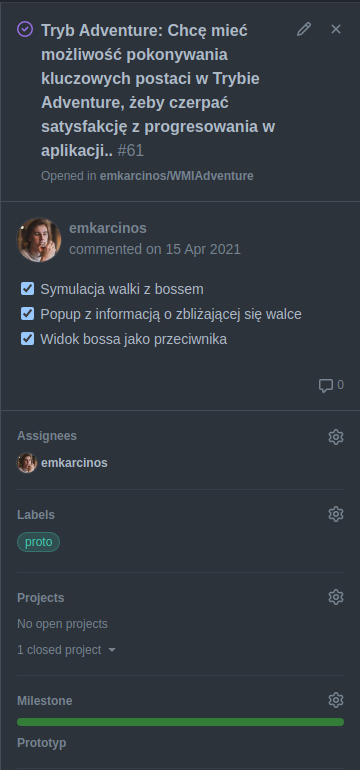
\includegraphics[scale=0.7]{card_initial_example.png}
    \newline
    Rys. 5 - Przykładowa Kanbanowa karteczka w pierwszej iteracji procesu - \url{https://github.com/emkarcinos/WMIAdventure/issues/61}
\end{center}

\subsection*{Stan z Grudnia 2021r.}
Link do tablicy na GitHub Projects: \url{https://github.com/emkarcinos/WMIAdventure/projects/12}

Cele sprintu są teraz dużo bardziej konkretnie określone.

\subsubsection*{Kolumny}
\begin{itemize}
    \item \textbf{Sprint Backlog} - Nowa kolumna w której trzymamy karteczki typu User Stories.
    \item \textbf{To do - do zrobienia} - w przeciwieństwie do pierwszej iteracji, w tej kolumnie przechowujemy tylko zadania programistyczne wykonywane w ramach danego sprintu
    \item \textbf{In progress - w trakcie pracy}
    \item \textbf{Testing and review - testowanie i recenzja} - wykonane zadania nie trafiały już od razu do sekcji "ukończone", tylko zawsze musiały przejść proces recenzji kodu oraz testowania.
    \item \textbf{Done - ukończone}
\end{itemize}
Główne różnice w tablicy wynikają z wprowadzenia dwóch nowych kolumn - \textit{Sprint Backlog} i \textit{Testing and review}.

Zaczęliśmy także stosować priorytetyzację kolumn - od prawej do lewej, to jest, zamiast rozpoczynać nowe zadania, zawsze powinniśmy najpiew przetestować zadania oczekujące na recenzję.

\subsubsection*{Karteczki - zadania}
Same karteczki przeszły największą metamorfozę. Ogólny podział karteczek na byty biznesowe (User Stories) i zadania drużynowe dalej obowiązuje, natomiast każda z tych dwóch katerogii została rozwinięta.

\subsubsection*{User Stories}
Karteczki tego typu dostały dwa oznaczenia: \textbf{User Story}, wyróżniające karteczkę w backlogu i \textbf{Story Points}, czyli abstrakcyjna wartość liczbowa reprezentująca poziom skomplikowania danego story.

W opisie danego User Story pojawiły się odniesienia do zadań programistycznych, które je realizują. Umożliwia to dokładne śledzenie procesu ukończenia danego celu biznesowego.

\begin{center}
    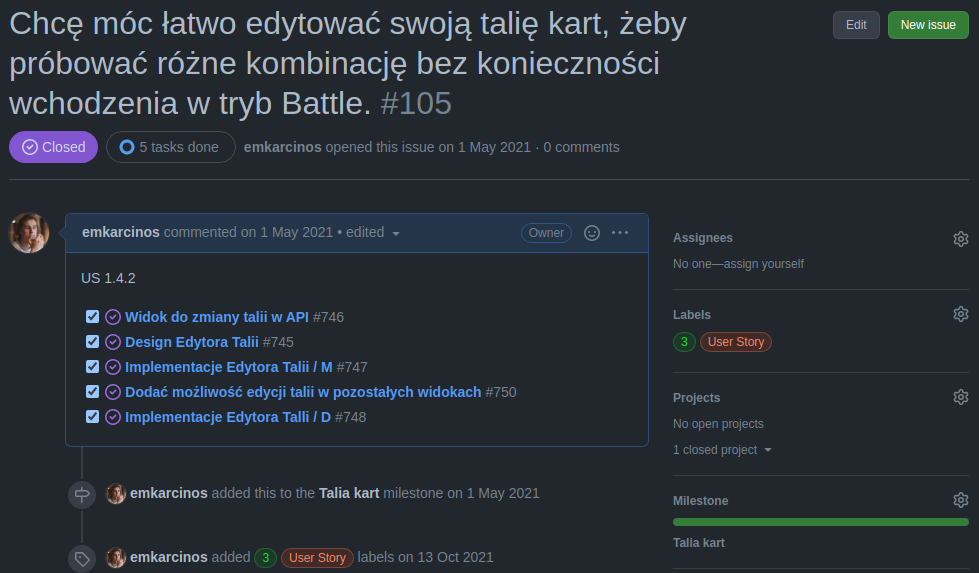
\includegraphics[scale=0.5]{card_user_story_example.png}
    \newline
    Rys. 6 - Przykładowa Kanbanowa karteczka typu User Story w końcowej iteracji procesu - \url{https://github.com/emkarcinos/WMIAdventure/issues/105}
\end{center}

\subsubsection*{Zadania programistyczne i inne}
Realizowanie User Stories jako zadania było niewygodne ze względu na to, że jeden User Story mógłby być realizowany przez więcej niż jeden sprint. Brakowało precyzji, którą osiągnęliśmy dzięki wprowadzaniu zadań typu programistycznego, lub typu innego (na przykład zdobycie nowej bazy danych, czy przygotowanie ankiety).

Zadania te często odnosiły się do konkretnych User Stories (wspominałem w sekcji wyżej - oznaczone jako podzadania).

Dodatkowo pojawiły się oznaczenia przy zadaniach sugerujące jakiej części systemu może dotyczyć (UI/UX, Frontend, backend). Wynikało to z naturalnego podziału na osoby bardziej specjalizujące się w danym obszarze systemu, przez co łatwiej wizualnie wybrać zadanie do realizacji.

\begin{center}
    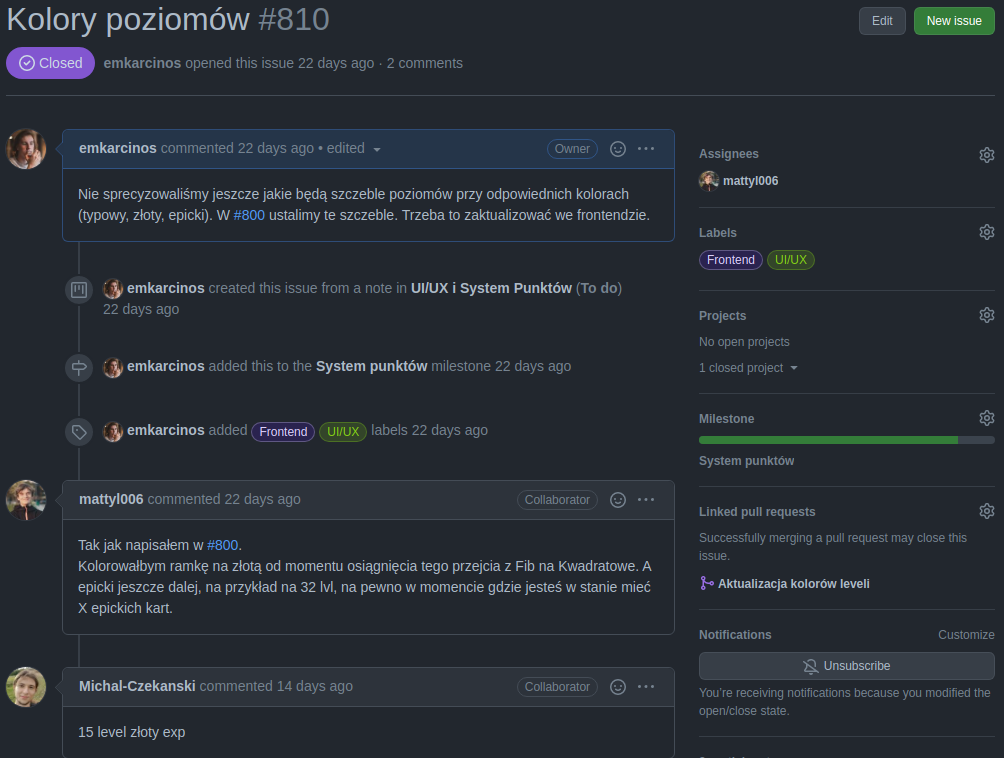
\includegraphics[scale=0.5]{card_implementation_task_example.png}
    \newline
    Rys. 7 - Przykładowa Kanbanowa karteczka z zadaniem programistycznym w końcowej iteracji procesu - \url{https://github.com/emkarcinos/WMIAdventure/issues/810}
\end{center}
\begin{center}
    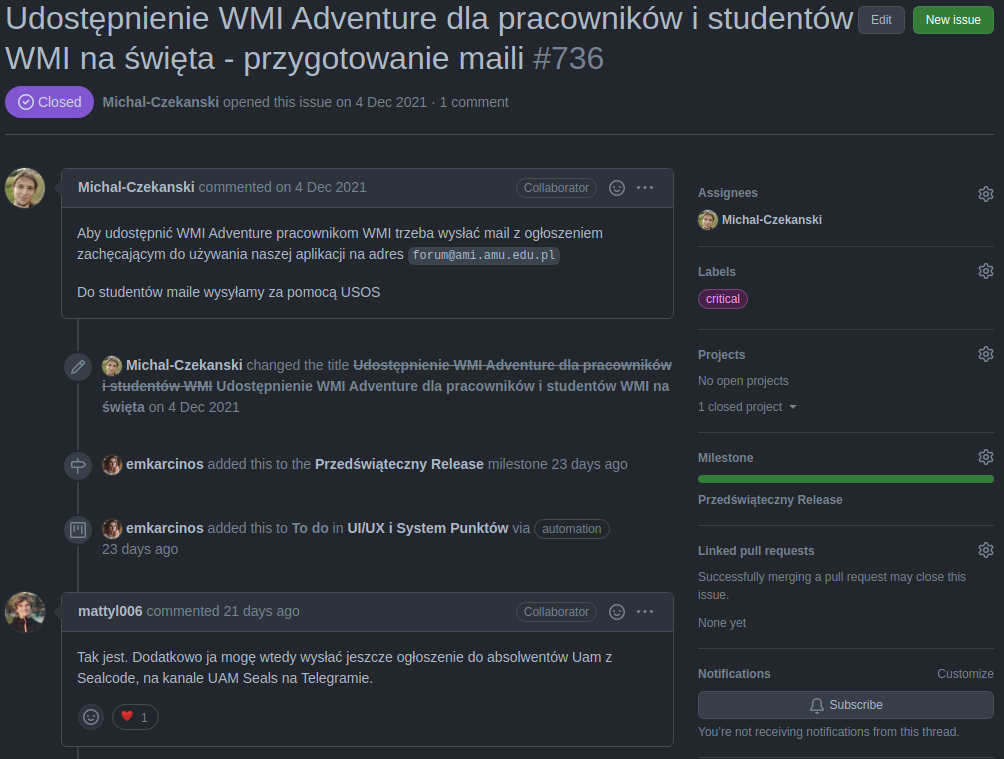
\includegraphics[scale=0.5]{card_other_task_example.png}
    \newline
    Rys. 8 - Przykładowa Kanbanowa karteczka z zadaniem nieprogramistycznym w końcowej iteracji procesu - \url{https://github.com/emkarcinos/WMIAdventure/issues/736}
\end{center}

\subsubsection*{Dyskusje pod karteczkami}
W nowej wersji procesu wprowadziliśmy większe dyskusje pod zadaniami na tablicy, aby skrócić bardzo długie codzienne spotkania i ułatwić planowanie. Każdy w ramach planowania miał zaznajomić się z zadanami, które wybraliśmy do realizacji w danym sprincie. Komentarze były miejscem na sugerowane rozwiązania i ewentualne pytania, dzięki czemu podczas ich wykonywania zespół był w stanie odnieść się do opinii i sugestii innych.

Dodatkowo wprowadziliśmy bardziej szerokie opisy zadań tak, aby były bardziej zrozumiałe dla osoby, która realizuje zadanie spoza swojego zakresu specjalności.

Jeżeli dana karteczka była poprarta dłuższą dyskusją, to decyzje i motywacje za nimi były także opisywane w treści zadania.

\subsubsection*{Zakres zadań}
Początkowo karteczki z zadaniami były bardzo obszerne i często wymagały wielu dni programistycznych na realizację. Chcieliśmy także móc pracować nad takimi zadanami asynchronicznie, dlatego zaczęliśmy rozdrabniać je na mniejsze fragmenty.

Zadania powinny być rozbijane na \textit{atomowe części} - poprawne rozbicie zadania na takie części umożliwia asynchroniczną pracę kilku członków zespołu bez kolizji. Mniejsze części powinny być niezależnie testowalne. Dodatkowo pomaga to zrozumieć skalę problemu danej karteczki.

\section{Wykorzystanie GitHub Projects jako narzędzia do zarządzania procesem}


\printbibliography

\end{document}
